\documentclass[11pt]{article}

\usepackage[a4paper,margin=1in]{geometry}
\usepackage{amsmath}
\usepackage{booktabs}
\usepackage{graphicx}
\usepackage{setspace}
\usepackage{natbib}
\usepackage[hidelinks]{hyperref}

\graphicspath{{../figures/}}
\onehalfspacing

\title{The Overnight Puzzle: Decomposing the Equity Premium into Overnight and Intraday Returns}
\author{Nafiz Noor}
\date{July 2026}

\begin{document}

\maketitle

\begin{abstract}
\noindent
I decompose the daily return on SPY, the S\&P 500 ETF, into an overnight leg (close to open) and an intraday leg (open to close) over 1 February 1993 to 14 July 2026, a sample of 8,419 trading days. Almost the entire equity premium accrues overnight: the overnight leg earns 9.99\% annualised at 10.60\% volatility (Sharpe 0.95), while the intraday leg earns 0.78\% at 15.21\% volatility (Sharpe 0.13); buy-and-hold earns 10.85\% (Sharpe 0.65). The split survives sub-period cuts and holds in QQQ, AAPL, MSFT, JPM, and even GLD, though the overnight leg also carries the crashes, losing 59.58\% annualised during the 2020 Covid drawdown. Trading it requires one round trip per day, and the breakeven round-trip cost is just 4.00 basis points. Net of realistic costs the strategy earns roughly nothing: the anomaly is a fact about when the equity premium accrues, not a tradeable strategy.
\end{abstract}

\section{Introduction}

The equity premium is usually measured close to close, as if the trading day were a single indivisible unit. It is not. Each day splits into two distinct regimes: roughly six and a half hours in which the market is open and prices are formed by continuous trading, and seventeen and a half hours (longer over weekends and holidays) in which the market is shut and prices can only jump from one day's close to the next day's open. There is no obvious reason the reward for bearing equity risk should be earned in one regime rather than the other. Yet it is.

This paper replicates and stress-tests the ``overnight anomaly'' on SPY, the S\&P 500 ETF, using daily open and close prices from 1 February 1993 to 14 July 2026 -- 8,419 trading days. The headline result is stark. The overnight leg, buying at each close and selling at the next open, earns 9.99\% annualised with a Sharpe ratio of 0.95. The intraday leg, buying at each open and selling at the same day's close, earns 0.78\% annualised with a Sharpe ratio of 0.13. The two legs compound exactly to the familiar buy-and-hold return of 10.85\% (Sharpe 0.65). Over thirty-three years, essentially all of the US equity premium in this instrument has accrued while the market was closed.

I then ask three follow-up questions. First, is the split robust? It is: it holds in both halves of the sample (though it weakens after 2010), and it appears in every asset I examine -- QQQ, AAPL, MSFT, JPM, and even the gold ETF GLD. It is not, however, a free lunch in the tails: the overnight leg carried the 2020 Covid crash, losing 59.58\% annualised over the 51-day drawdown window, and was negative through 2022. Second, can it be traded? Mechanically yes, economically no. The naive implementation trades one round trip per day, roughly 252 per year, and the mean overnight return of 4.00 basis points per day is therefore also the breakeven round-trip cost. There is no realistic retail execution path below about 2 basis points once the bid--ask spread is crossed twice daily, and at 2 basis points the net Sharpe ratio has already fallen below buy-and-hold. Third, does conditioning help? Modestly: overnight returns are higher after down days and lower after strong up days, consistent with short-horizon reversal, and both legs are elevated on scheduled FOMC announcement days, consistent in spirit with the pre-FOMC drift of \citet{lucca2015}.

The contribution is deliberately modest. This is a careful replication on public data, with attention to two traps that can silently corrupt the decomposition -- dividend adjustment and stale opening prints -- plus an honest accounting of transaction costs. The conclusion I draw is the one the cost arithmetic forces: the overnight anomaly is best read as a striking fact about \emph{when} the equity premium accrues, not as a strategy.

The rest of the paper proceeds as follows. Section~\ref{sec:lit} places the exercise in the literature. Section~\ref{sec:data} describes the data, the return definitions, and the data-quality checks. Section~\ref{sec:anomaly} presents the headline decomposition. Section~\ref{sec:robust} reports sub-period and cross-asset robustness. Section~\ref{sec:trading} works through the cost arithmetic. Section~\ref{sec:conditional} presents two conditional cuts. Section~\ref{sec:conclusion} concludes.

\section{Related literature}
\label{sec:lit}

The night--day return split was first documented systematically by \citet{cooper2008}, who showed that the US equity premium over 1993--2006 was earned almost entirely in the overnight session, with intraday returns close to zero. \citet{lou2019} extended the fact to the cross-section: characteristic-based strategies display a ``tug of war'' in which overnight and intraday components of the same anomaly returns systematically offset, which they attribute to distinct investor clienteles trading at the open and at the close. \citet{hendershott2020} sharpened the asset-pricing content of the split, showing that the CAPM performs well overnight -- beta is positively priced close to open -- and fails intraday, where the beta--return relation is flat or negative. Relative to these papers, my exercise is narrow: a single-index replication with modern data through 2026, plus cost and conditioning analysis.

Two further strands are relevant. \citet{lucca2015} document that a large share of the equity premium is earned in the 24 hours before scheduled FOMC announcements; since much of that window falls outside regular trading hours, the pre-FOMC drift and the overnight anomaly plausibly overlap, and Section~\ref{sec:conditional} runs a light check on FOMC days in my sample. Finally, \citet{knuteson2020} argues that the persistence and ubiquity of the overnight--intraday split is so strange that it hints at systematic price manipulation. I cite the paper as a provocation rather than an explanation: the patterns documented here are consistent with far more prosaic mechanisms -- inventory risk premia, clientele effects, and the mechanical placement of news and dividends in the overnight window -- and nothing in my results requires a manipulative account.

\section{Data and method}
\label{sec:data}

\subsection{Data}

I download daily open, high, low, and close prices from Yahoo Finance via the \texttt{yfinance} Python package. The main series is SPY, the S\&P 500 ETF, from 1 February 1993 (shortly after the fund's launch) to 14 July 2026, giving 8,419 daily return observations. Section~\ref{sec:robust} repeats the analysis on QQQ, AAPL, MSFT, JPM, and GLD, using each ticker's full available history: AAPL, MSFT, and JPM from January 1993, QQQ from March 1999, GLD from November 2004. The full pipeline, from download to every table and figure in this paper, is reproducible from a single script.

All prices are downloaded with \texttt{auto\_adjust=True}, so that dividends and splits are folded into the open \emph{and} the close consistently. This choice is not cosmetic. Dividends go ex-dividend at the open, so the cash lands in the overnight gap: an ex-dividend day mechanically prints a lower open against the previous close. Mixing an adjusted close with an unadjusted open -- an easy mistake with vendor data, where ``adjusted close'' is often the only adjusted field -- would push SPY's roughly 2\% dividend yield out of the overnight leg and corrupt the decomposition by an amount comparable to the effect being measured. Using a consistently adjusted OHLC panel keeps the dividend where it economically belongs: in the close-to-open return.

\subsection{Return definitions and conventions}

Let $O_t$ and $C_t$ denote the (adjusted) open and close on day $t$. The overnight and intraday returns are
\begin{equation}
r^{\text{on}}_t = \frac{O_t}{C_{t-1}} - 1,
\qquad
r^{\text{in}}_t = \frac{C_t}{O_t} - 1,
\end{equation}
and by construction the two legs compound exactly to the close-to-close daily return:
\begin{equation}
(1 + r^{\text{on}}_t)(1 + r^{\text{in}}_t) = \frac{C_t}{C_{t-1}} = 1 + r^{\text{daily}}_t.
\end{equation}
The decomposition is therefore an identity, not a model: every basis point of the daily return is assigned to exactly one leg.

Throughout, annualised returns are geometric (a CAGR computed from the compounded daily series, annualised at 252 trading days per year), annualised volatility is the daily standard deviation multiplied by $\sqrt{252}$, and Sharpe ratios are the daily mean over the daily standard deviation, multiplied by $\sqrt{252}$, with the risk-free rate set to zero. The zero risk-free convention is a genuine limitation, discussed in Section~\ref{sec:conclusion}: it flatters all three series equally in level terms but does not affect the comparison between legs, which is the object of interest.

\subsection{A stale-open check}
\label{sec:stale}

The decomposition leans entirely on the quality of the opening print, which is the weakest field in free vendor data. A ``stale'' open -- the open recorded as identical to the previous close, as happened in some older feeds when no opening trade was captured -- produces an overnight return of exactly zero and silently shifts that day's entire return into the intraday leg. As a diagnostic, Table~\ref{tab:quality} reports the share of days on which SPY's recorded overnight return is exactly zero, by decade.

\begin{table}[t]
\centering
\caption{Share of SPY trading days with an exactly-zero overnight return, by decade. An exactly-zero overnight return is a proxy for a stale opening print (open recorded equal to the previous close), which shifts that day's entire return into the intraday leg.}
\label{tab:quality}
\begin{tabular}{lr}
\toprule
Decade & Share of days with zero overnight return (\%) \\
\midrule
1990s & 5.43 \\
2000s & 1.03 \\
2010s & 1.27 \\
2020s & 0.24 \\
\bottomrule
\end{tabular}
\end{table}

The pattern is what one would hope for: 5.43\% of days in the 1990s, falling to 0.24\% in the 2020s as opening auctions and data capture improved. Two remarks follow. First, the problem is real but small: even in the worst decade, nineteen days in twenty have a distinct opening print. Second, and more usefully, the direction of the bias works \emph{against} the anomaly. A stale open moves return from the overnight leg to the intraday leg, so if anything the true overnight--intraday gap in the early sample is slightly wider than measured here. I make no correction and simply flag the caveat: Yahoo's early opens are imperfect, and the decade-level split in the early 1990s should be read with that in mind.

\section{The anomaly}
\label{sec:anomaly}

Table~\ref{tab:headline} reports the headline decomposition for SPY over the full sample, and Figure~\ref{fig:wealth} shows the corresponding wealth curves: the growth of \pounds 1 invested, on a log scale, in the overnight leg only, the intraday leg only, and buy-and-hold.

\begin{table}[t]
\centering
\caption{Decomposition of SPY daily returns, 1 February 1993 to 14 July 2026 (8,419 trading days). Overnight is close to open, intraday is open to close; the two legs compound to the daily close-to-close return. Annualised returns are geometric (CAGR); volatility is the daily standard deviation scaled by $\sqrt{252}$; Sharpe ratios assume a zero risk-free rate.}
\label{tab:headline}
\begin{tabular}{lrrr}
\toprule
 & Ann.\ return (\%) & Ann.\ vol.\ (\%) & Sharpe \\
\midrule
Overnight (close $\to$ open) & 9.99 & 10.60 & 0.95 \\
Intraday (open $\to$ close) & 0.78 & 15.21 & 0.13 \\
Daily (close $\to$ close) & 10.85 & 18.57 & 0.65 \\
\bottomrule
\end{tabular}
\end{table}

\begin{figure}[t]
\centering
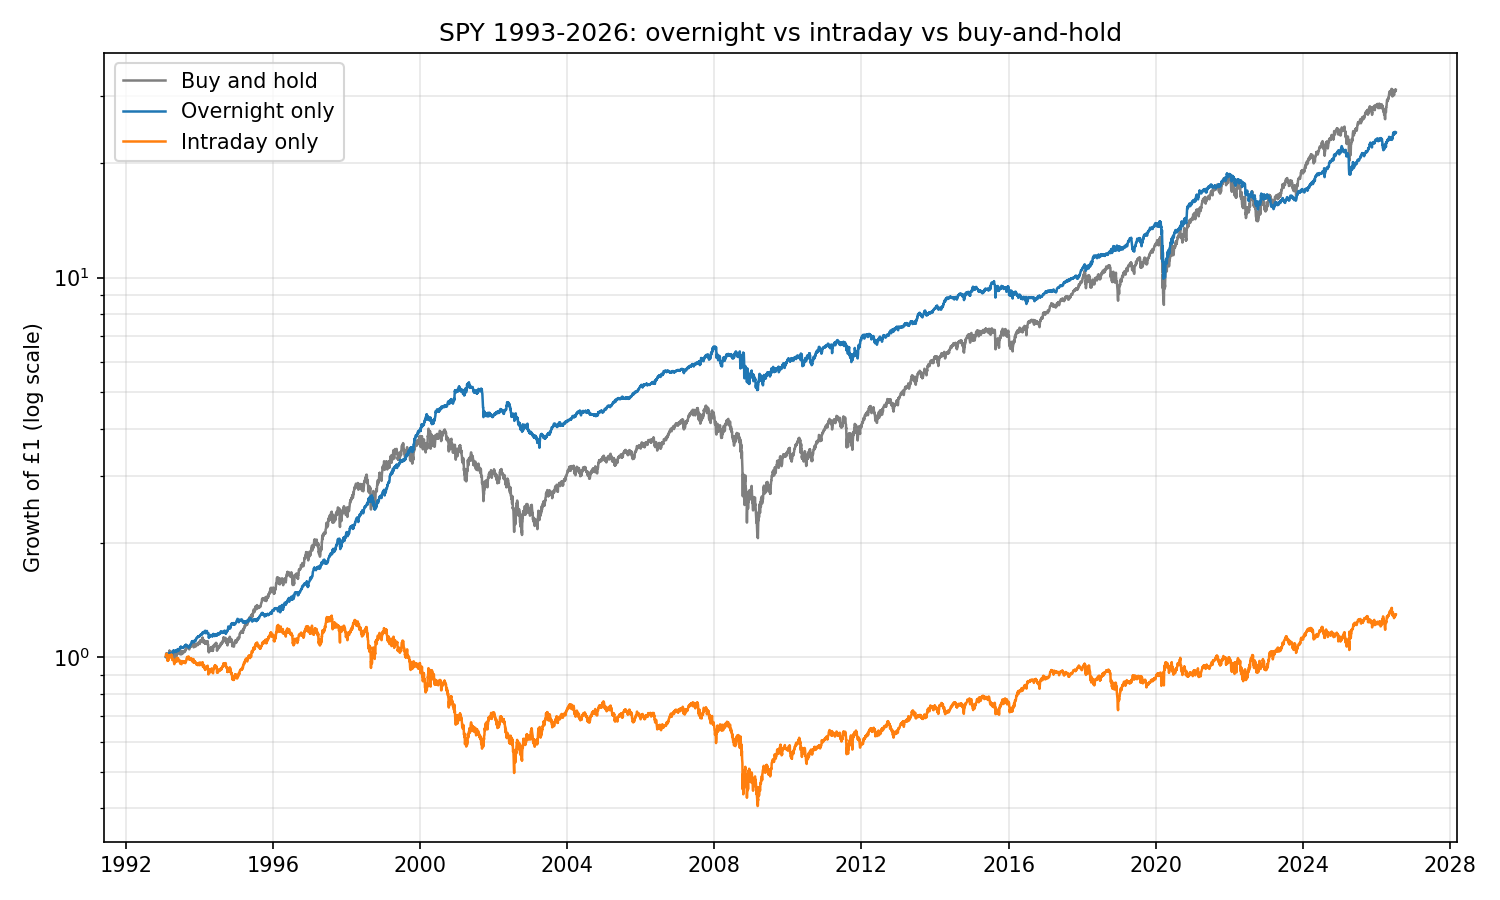
\includegraphics[width=\textwidth]{spy_wealth_curves.png}
\caption{Growth of \pounds 1 in SPY, 1993--2026, on a log scale: overnight leg only (buy every close, sell every open), intraday leg only (buy every open, sell every close), and buy-and-hold. The overnight curve captures essentially all of buy-and-hold's cumulative growth at visibly lower volatility; the intraday curve is roughly flat for three decades. Returns are before transaction costs.}
\label{fig:wealth}
\end{figure}

The numbers speak plainly. An investor who held SPY only while the market was closed earned 9.99\% a year for thirty-three years; an investor who held it only while the market was open earned 0.78\% a year over the same period. The overnight leg alone delivers essentially the entire buy-and-hold return of 10.85\%, and it does so at 10.60\% annualised volatility against buy-and-hold's 18.57\%, which is why its Sharpe ratio of 0.95 comfortably exceeds buy-and-hold's 0.65. The intraday leg, despite carrying the larger share of the volatility (15.21\%), earns a Sharpe ratio of just 0.13.

Two features of Table~\ref{tab:headline} deserve a remark. First, most volatility is realised while the market is open, even though the overnight window covers far more clock time, including every weekend and holiday: trading itself generates variance. Second, the legs' volatilities of 10.60\% and 15.21\% combine in quadrature to almost exactly the daily figure of 18.57\%, so the two legs are close to uncorrelated -- the decomposition really does split the day into two distinct return-generating regimes rather than two noisy copies of one regime.

Figure~\ref{fig:wealth} makes the same point visually and adds the time dimension. The overnight curve tracks the buy-and-hold curve's long-run drift while cutting through its drawdowns less violently; the intraday curve wanders around \pounds 1 for three decades. Whatever the equity premium is compensation for, in this sample it was paid out between the closing bell and the next opening print.

\section{Robustness}
\label{sec:robust}

A split this stark invites two immediate suspicions: that it is an artefact of one peculiar era, or an artefact of one peculiar instrument. This section addresses both.

\subsection{Sub-periods}

Table~\ref{tab:subperiods} splits the SPY sample at the end of 2009 and adds two stress windows: the Covid crash (19 February to 30 April 2020) and the calendar year 2022.

\begin{table}[t]
\centering
\caption{SPY overnight and intraday legs by sub-period. Annualised returns are geometric; Sharpe ratios assume a zero risk-free rate. Figures for the two short windows are annualised from 51 and 251 trading days respectively and should be read as descriptive, not as expected returns.}
\label{tab:subperiods}
\begin{tabular}{lrrrrr}
\toprule
 & \multicolumn{2}{c}{Overnight} & \multicolumn{2}{c}{Intraday} & \\
\cmidrule(lr){2-3}\cmidrule(lr){4-5}
Period & Ann.\ ret.\ (\%) & Sharpe & Ann.\ ret.\ (\%) & Sharpe & Days \\
\midrule
1993--2009 & 11.26 & 1.09 & $-3.29$ & $-0.11$ & 4,263 \\
2010--2026 & 8.71 & 0.82 & 5.13 & 0.45 & 4,156 \\
2020 crash (19 Feb--30 Apr) & $-59.58$ & $-1.62$ & 22.74 & 0.79 & 51 \\
2022 & $-13.39$ & $-0.98$ & $-5.60$ & $-0.19$ & 251 \\
\bottomrule
\end{tabular}
\end{table}

The effect is strongest in the first half of the sample. From 1993 to 2009 the overnight leg earned 11.26\% annualised (Sharpe 1.09) while the intraday leg \emph{lost} 3.29\% a year -- for seventeen years, holding the S\&P 500 only during trading hours was a losing proposition. After 2010 the gap narrows: the overnight leg still dominates at 8.71\% (Sharpe 0.82), but the intraday leg turns respectable at 5.13\% (Sharpe 0.45). Whether the post-2010 softening reflects the anomaly's publication (\citealp{cooper2008}; \citealp{lou2019}), structural change in overnight trading, or the cleaner opening prints documented in Section~\ref{sec:stale} feeding less return into the overnight leg, this design cannot say.

The stress windows carry the more important lesson. During the Covid crash the overnight leg lost 59.58\% annualised over 51 trading days (Sharpe $-1.62$) while the intraday leg actually gained, at an annualised 22.74\%. In 2022 the overnight leg lost 13.39\% against the intraday leg's $-5.60$\%. The pattern is coherent: the overnight session is when news lands and gaps happen, so the leg that harvests the premium in calm times is also the leg that absorbs the crashes. The overnight anomaly is not a low-risk arbitrage; it is a risk premium with a left tail, concentrated in the hours when the holder cannot trade out of the position.

\subsection{Other assets}

Table~\ref{tab:assets} runs the identical decomposition on five further tickers over each one's full available history, and Figure~\ref{fig:assets} plots the annualised return of each leg by asset.

\begin{table}[t]
\centering
\caption{Overnight versus intraday decomposition by asset, each over its full available Yahoo Finance history (start date shown). Annualised returns are geometric; Sharpe ratios assume a zero risk-free rate. All prices are adjusted for dividends and splits.}
\label{tab:assets}
\begin{tabular}{llrrrrr}
\toprule
 & & \multicolumn{2}{c}{Overnight} & \multicolumn{2}{c}{Intraday} & \\
\cmidrule(lr){3-4}\cmidrule(lr){5-6}
Asset & From & Ann.\ ret.\ (\%) & Sharpe & Ann.\ ret.\ (\%) & Sharpe & Days \\
\midrule
SPY & 1993-02-01 & 9.99 & 0.95 & 0.78 & 0.13 & 8,419 \\
QQQ & 1999-03-11 & 13.88 & 0.98 & $-2.63$ & $-0.00$ & 6,877 \\
AAPL & 1993-01-05 & 21.90 & 0.91 & $-0.03$ & 0.17 & 8,438 \\
MSFT & 1993-01-05 & 10.61 & 0.67 & 6.47 & 0.37 & 8,438 \\
JPM & 1993-01-05 & 10.82 & 0.63 & 2.42 & 0.23 & 8,438 \\
GLD & 2004-11-19 & 10.65 & 0.85 & $-0.28$ & 0.04 & 5,444 \\
\bottomrule
\end{tabular}
\end{table}

\begin{figure}[t]
\centering
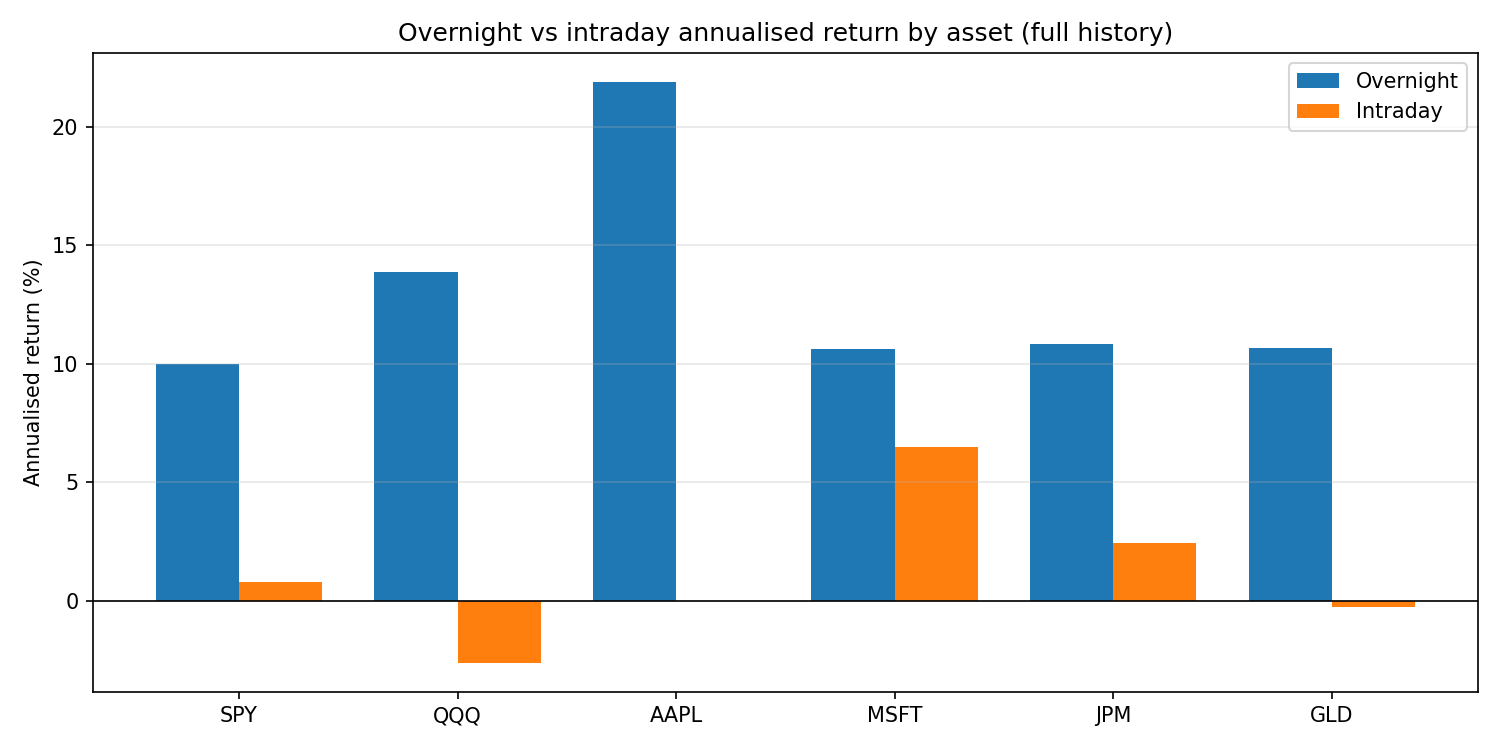
\includegraphics[width=\textwidth]{asset_decomposition.png}
\caption{Annualised overnight and intraday returns by asset, each over its full available history (QQQ from 1999, GLD from 2004, others from 1993). The overnight leg dominates in every asset examined, including the gold ETF GLD.}
\label{fig:assets}
\end{figure}

The split holds everywhere. It is most extreme in the growth-heavy names: QQQ earned 13.88\% a year overnight against $-2.63$\% intraday since 1999, and AAPL earned a remarkable 21.90\% overnight against $-0.03$\% intraday since 1993 -- three decades of Apple's compounding, delivered almost entirely between sessions. (AAPL's intraday leg shows a slightly negative CAGR alongside a small positive Sharpe of 0.17; the arithmetic daily mean is positive but volatility drag on a single high-variance stock pushes the geometric return just below zero.) The split is narrowest, though still present, in MSFT (10.61\% overnight versus 6.47\% intraday) and JPM (10.82\% versus 2.42\%).

The most interesting row is GLD. Gold is not an equity, pays no dividend, and carries no obvious claim to the equity risk premium, yet its overnight leg earned 10.65\% annualised (Sharpe 0.85) against an intraday leg of $-0.28$\% since 2004. That the same night--day asymmetry appears in a commodity ETF suggests the anomaly is not purely a story about where the \emph{equity} premium sits in the day. It points instead towards mechanisms that operate on any exchange-traded instrument: compensation for bearing inventory and gap risk through the non-trading hours, and systematic differences between the investor clienteles active at the open and at the close, the mechanisms emphasised by \citet{hendershott2020} and \citet{lou2019} respectively.

\section{Trading the anomaly}
\label{sec:trading}

The wealth curves in Figure~\ref{fig:wealth} describe a paper portfolio. The natural question is whether the overnight leg can actually be captured. The naive implementation is mechanical: buy at every close, sell at every open. That is one round trip per day, roughly 252 per year, and this trading intensity -- not the size of the premium -- is what decides the question.

The arithmetic is unforgiving. With about 252 round trips a year, each basis point of round-trip cost drains roughly 252 basis points, about 2.52 percentage points, of annual return (slightly more once compounding is accounted for, as the sweep below shows). Against that stands a mean overnight return of 4.00 basis points per day. The mean daily return \emph{is} the breakeven round-trip cost: at 4.00 basis points per round trip, the strategy's net mean return is zero by construction.

Table~\ref{tab:costs} sweeps the round-trip cost from zero to 5 basis points, and Figure~\ref{fig:costs} plots the net Sharpe ratio against cost with the breakeven marked.

\begin{table}[t]
\centering
\caption{Net performance of the naive overnight strategy on SPY (buy every close, sell every open; one round trip per day, roughly 252 per year) as a function of the assumed round-trip transaction cost. The cost is deducted from every day's overnight return. Annualised returns are geometric; Sharpe ratios assume a zero risk-free rate. The breakeven round-trip cost equals the mean overnight return of 4.00 basis points per day.}
\label{tab:costs}
\begin{tabular}{rrr}
\toprule
Round-trip cost (bps) & Net ann.\ return (\%) & Net Sharpe \\
\midrule
0.0 & 9.99 & 0.95 \\
0.5 & 8.61 & 0.83 \\
1.0 & 7.25 & 0.71 \\
1.5 & 5.91 & 0.60 \\
2.0 & 4.59 & 0.48 \\
2.5 & 3.28 & 0.36 \\
3.0 & 1.98 & 0.24 \\
3.5 & 0.71 & 0.12 \\
4.0 & $-0.55$ & 0.00 \\
4.5 & $-1.80$ & $-0.12$ \\
5.0 & $-3.03$ & $-0.24$ \\
\bottomrule
\end{tabular}
\end{table}

\begin{figure}[t]
\centering
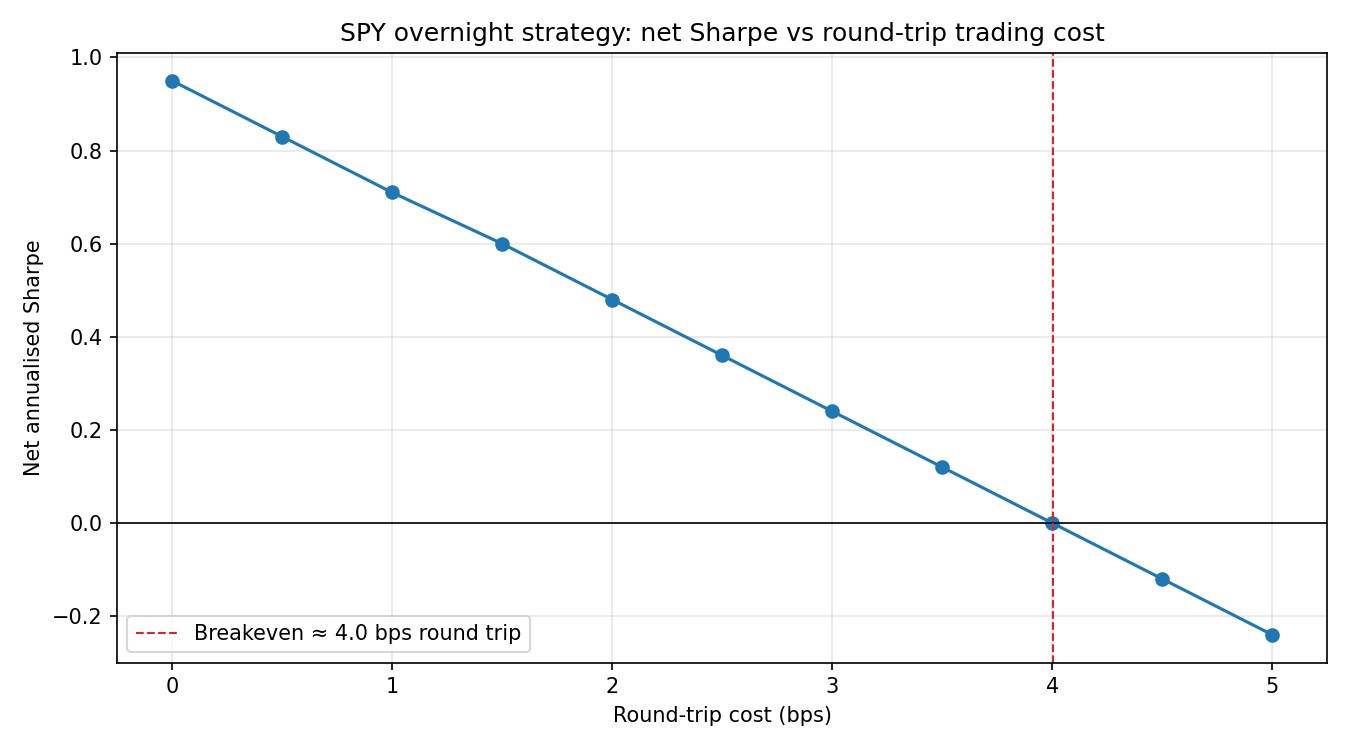
\includegraphics[width=\textwidth]{net_sharpe_vs_cost.png}
\caption{Net Sharpe ratio of the naive overnight strategy on SPY as a function of the assumed round-trip cost, with the breakeven cost of 4.00 basis points marked. Each basis point of round-trip cost removes roughly 2.52 percentage points of annual return.}
\label{fig:costs}
\end{figure}

The verdict deserves stating plainly: \emph{the anomaly survives only if round-trip costs are under about 4 basis points, and there is no realistic retail path below roughly 2 basis points once the spread is crossed twice a day and commissions are paid -- so net of realistic costs, the tradeable version earns roughly nothing.} SPY is among the most liquid securities in the world, with a typical quoted spread of one cent on a price of several hundred dollars, but crossing even that spread twice a day, every day, plus any commission, regulatory fees, and the slippage of transacting at or around the opening and closing auctions, makes an all-in round-trip cost below 2 basis points implausible for a retail account. At 2 basis points the strategy nets 4.59\% a year at a Sharpe ratio of 0.48 -- already below buy-and-hold's 0.65, with 252 times the trading. At 3 basis points it nets 1.98\%; at the 4.00 basis point breakeven it nets $-0.55$\% (the geometric return sits just below zero when the arithmetic mean is exactly zero).

This sweep is, if anything, generous to the strategy. It ignores taxes on short-term gains, assumes execution exactly at the official close and open, and prices no compensation for the operational burden of two orders a day for thirty-three years. A sophisticated institution paying near-zero commissions and providing rather than taking liquidity might approach the breakeven; a retail investor cannot. The economics here echo the broader point in \citet{lou2019}: night--day return gaps can be large and persistent precisely because the cost of harvesting them at daily frequency roughly exhausts them.

\section{Conditional evidence}
\label{sec:conditional}

Two cheap conditional cuts sharpen the picture of what the overnight return is. Both are descriptive, in-sample splits with simple $t$-statistics; neither is a formal study.

\subsection{Conditioning on the previous day}

Table~\ref{tab:prevday} buckets each night's overnight return by the same day's close-to-close return -- that is, tonight's gap conditioned on today's full-day move.

\begin{table}[t]
\centering
\caption{SPY mean overnight return (in basis points) conditional on the same day's close-to-close return, 1993--2026. The $t$-statistic tests the mean of each bucket against zero and makes no adjustment for heteroskedasticity or overlapping information; these are descriptive splits, not formal tests.}
\label{tab:prevday}
\begin{tabular}{lrrr}
\toprule
Today's daily return & Mean overnight (bps) & $t$-stat & Days \\
\midrule
$<-2\%$ & 8.02 & 1.08 & 337 \\
$-2\%$ to $-1\%$ & 7.65 & 2.41 & 718 \\
$-1\%$ to $0\%$ & 5.41 & 5.21 & 2,810 \\
$0\%$ to $1\%$ & 3.69 & 4.30 & 3,379 \\
$1\%$ to $2\%$ & $-0.17$ & $-0.07$ & 900 \\
$>2\%$ & $-7.37$ & $-0.97$ & 274 \\
\bottomrule
\end{tabular}
\end{table}

The pattern declines nearly monotonically across the buckets: overnight returns average around 8 basis points after down days and fall to $-7.37$ basis points after days that gained more than 2\%. The means are statistically distinguishable from zero in the middle buckets, where the samples are large ($t$-statistics of 5.21 and 4.30 in the two central bins, 2.41 in the $-2\%$ to $-1\%$ bin), but not in the tails, where the bins hold only a few hundred high-volatility days ($t$-statistics of 1.08 and $-0.97$). The natural reading is short-horizon reversal layered on top of the base effect: the unconditional overnight premium of about 4 basis points is amplified after selling pressure and extinguished -- perhaps reversed -- after strong rallies. I resist reading more into the tails than the $t$-statistics permit.

\subsection{FOMC announcement days}

Table~\ref{tab:fomc} splits the sample around scheduled FOMC announcements. I compiled the announcement dates from the Federal Reserve's official meeting calendars: 259 scheduled statement-release days from February 1994 to June 2026, where the announcement day is the final day of each scheduled meeting; unscheduled meetings and conference calls are excluded.

\begin{table}[t]
\centering
\caption{SPY mean overnight and intraday returns (in basis points) around scheduled FOMC announcements, 1994--2026. Announcement days are the 259 statement-release days of scheduled meetings, compiled from the Federal Reserve's official calendars; unscheduled meetings and conference calls are excluded. The announcement day is the final day of the meeting.}
\label{tab:fomc}
\begin{tabular}{lrrr}
\toprule
 & Mean overnight (bps) & Mean intraday (bps) & Days \\
\midrule
FOMC announcement day & 13.38 & 11.17 & 259 \\
Day after FOMC & 1.56 & $-3.83$ & 257 \\
All other days & 3.78 & 0.58 & 7,903 \\
\bottomrule
\end{tabular}
\end{table}

Announcement days are unusually good for both legs: the overnight return averages 13.38 basis points against 3.78 on ordinary days, and the intraday return averages 11.17 basis points against 0.58. The elevated overnight figure -- the gap into the morning of the announcement -- sits comfortably alongside the pre-FOMC announcement drift of \citet{lucca2015}, who show that a striking share of the equity premium is earned in the 24 hours before the 2 p.m.\ statement, a window that spans exactly this overnight session and the pre-announcement hours of the trading day. The day after the announcement looks ordinary or slightly worse (1.56 basis points overnight, $-3.83$ intraday). I stress the limits of this cut: 259 event days is a small sample, no test statistics are reported, and this is a light conditional check on the anomaly rather than a study of the drift itself. What it establishes is modest but useful -- the overnight premium is not \emph{merely} a repackaged FOMC effect, since it averages a healthy 3.78 basis points on the 7,903 days with no announcement anywhere nearby.

\section{Conclusion}
\label{sec:conclusion}

Over 8,419 trading days from 1993 to 2026, essentially the entire equity premium in SPY was earned while the market was closed: 9.99\% a year overnight (Sharpe 0.95) against 0.78\% a year intraday (Sharpe 0.13). The fact is robust in the ways that matter. It holds in both halves of the sample, though it softens after 2010 as the intraday leg recovers to 5.13\%. It holds in every asset examined, from QQQ and AAPL at the extreme to MSFT and JPM at the narrow end, and it holds in GLD, which suggests the mechanism is at least partly about the microstructure of holding exchange-traded instruments through non-trading hours rather than about equities as such. And it is not a statistical fluke of calm markets: the overnight leg absorbed the 2020 crash at $-59.58$\% annualised and lost money throughout 2022. The premium and the risk live in the same hours.

The implementability verdict is unambiguous. Harvesting the overnight leg requires a round trip every day, the breakeven round-trip cost is 4.00 basis points, and each basis point of cost removes roughly 2.52 percentage points of annual return. No retail execution path plausibly gets below about 2 basis points all-in, at which point the net Sharpe ratio of 0.48 already trails simple buy-and-hold. The overnight anomaly, on this evidence, is a fact about \emph{when} the equity premium accrues -- a fact any theory of the premium ought to confront -- and not a strategy.

Several limitations bound these conclusions. The data are free Yahoo Finance feeds, and the opening prints in the early sample are imperfect: 5.43\% of days in the 1990s show an exactly-zero overnight return consistent with a stale open, though the resulting bias works against the anomaly rather than for it. Sharpe ratios assume a zero risk-free rate, which overstates all risk-adjusted figures in level terms, particularly over the high-rate portions of the sample. The cost analysis models proportional costs only, and prices none of the risks specific to running the strategy at scale -- overnight gap risk that cannot be exited, financing, taxes, or borrow considerations for any short-side variant. Everything is in-sample and descriptive, and the only statistical evidence offered is simple unadjusted $t$-statistics on conditional means. Within those bounds, the replication is clean, and the puzzle stands: for thirty-three years, the market has paid its equity holders mostly for the hours when nobody could trade.

\begin{thebibliography}{9}

\bibitem[Cooper et~al.(2008)Cooper, Cliff, and Gulen]{cooper2008}
Cooper, M.~J., Cliff, M.~T., and Gulen, H. (2008).
Return differences between trading and non-trading hours: Like night and day.
Working paper, SSRN.

\bibitem[Hendershott et~al.(2020)Hendershott, Livdan, and R\"osch]{hendershott2020}
Hendershott, T., Livdan, D., and R\"osch, D. (2020).
Asset pricing: A tale of night and day.
\emph{Journal of Financial Economics}, 138(3), 635--662.

\bibitem[Knuteson(2020)]{knuteson2020}
Knuteson, B. (2020).
Strikingly suspicious overnight and intraday returns.
Working paper, arXiv.

\bibitem[Lou et~al.(2019)Lou, Polk, and Skouras]{lou2019}
Lou, D., Polk, C., and Skouras, S. (2019).
A tug of war: Overnight versus intraday expected returns.
\emph{Journal of Financial Economics}, 134(1), 192--213.

\bibitem[Lucca and Moench(2015)]{lucca2015}
Lucca, D.~O., and Moench, E. (2015).
The pre-FOMC announcement drift.
\emph{Journal of Finance}, 70(1), 329--371.

\end{thebibliography}

\end{document}
